%% =====================================================================
%% uFlow: Software publication for SoftwareX (Elsevier)
%% Template: Original Software Publication (OSP)
%% Word limit: 4000 (target ~3000); Figures: max 6
%% =====================================================================
\documentclass[preprint,12pt,a4paper]{elsarticle}

\usepackage{amssymb}
\usepackage{amsmath}
\usepackage{hyperref}
\usepackage{graphicx}
\usepackage{booktabs}
\usepackage{siunitx}
\usepackage{listings}
\usepackage{xcolor}
\setlength{\parindent}{0pt}

\sisetup{per-mode=symbol,range-phrase=--,range-units=single}
\DeclareSIUnit\decibel{dB}
\DeclareSIUnit\minute{min}

\lstset{
  basicstyle=\ttfamily\footnotesize,
  breaklines=true,
  showstringspaces=false,
  language=Java, % closest to JS in listings
  commentstyle=\color{gray!70!black},
  keywordstyle=\color{blue!70!black}
}

\journal{SoftwareX}

\begin{document}
\renewcommand{\labelenumii}{\arabic{enumi}.\arabic{enumii}}

\begin{frontmatter}

\title{$\mu$Flow: An interactive browser-based 3D simulator for microfluidic Hall-effect magnetic bead detection}

\author[rutgers]{Harshitha Govindaraju\corref{cor1}}
\ead{harshitha.govindaraju@rutgers.edu}

\author[rutgers]{Umer Hassan}
\ead{umer.hassan@rutgers.edu}

\cortext[cor1]{Corresponding author.}

\address[rutgers]{Department of Electrical and Computer Engineering, Rutgers, The State University of New Jersey, 94 Brett Road, Piscataway, NJ 08854, USA}

\begin{abstract}
$\mu$Flow is a browser-based 3D interactive simulator for microfluidic Hall-effect detection of superparamagnetic beads. The tool couples four analytical physics modules (Clausius--Mossotti bead magnetization with volume-fraction correction, point-dipole stray field, volume-averaged Hall voltage with geometric correction, and Poiseuille flow with adaptive sub-stepping) together with a thermal $1/f$ noise framework across a database of 12 sensor platforms spanning graphene, III--V semiconductors, Si CMOS, bismuth, and topological insulators. The analytical model reproduces the COMSOL FEM-BEM benchmark from our companion study to within \SI{4.8}{\percent} at the favorable bead-to-sensor area ratio of Design~II, with the known point-dipole near-field limit at $h/R=1$ producing larger deviations (\SI{22}{\percent} and \SI{15}{\percent}) at the off-optimum Designs~I and~III, consistent with Jenkins et al.\ (2019). A built-in 2D axisymmetric magnetostatic FEM solver provides an independent volumetric-field check on the dipole model. A parametric sweep engine evaluates thousands of configurations in seconds, and a batch mode collects per-bead detection statistics under Poiseuille flow. $\mu$Flow is a single HTML file requiring no installation, build step, or commercial license.
\end{abstract}

\begin{keyword}
microfluidic simulation \sep Hall-effect sensor \sep magnetic bead detection \sep biosensor design \sep browser-based visualization \sep parametric optimization
\end{keyword}

\end{frontmatter}

% =====================================================================
\section*{Required Metadata}
\section*{Current code version}
% =====================================================================

\begin{table}[!h]
\centering
\footnotesize
\begin{tabular}{|l|p{6.0cm}|p{6.0cm}|}
\hline
\textbf{Nr.} & \textbf{Code metadata description} & \textbf{Value} \\
\hline
C1 & Current code version & v1.0 \\
\hline
C2 & Permanent link to code/repository used for this code version & \url{https://github.com/hg293/microfluidic-hall-sensor} \\
\hline
C3 & Permanent link to Reproducible Capsule & N/A \\
\hline
C4 & Legal Code License & MIT \\
\hline
C5 & Code versioning system used & git \\
\hline
C6 & Software code languages, tools, and services used & JavaScript (ES2020), HTML5, CSS3, React 18 (UMD), Three.js r160 (WebGL), HTML5 Canvas 2D \\
\hline
C7 & Compilation requirements, operating environments \& dependencies & Modern web browser with WebGL~2 support (Chrome 90+, Firefox 88+, Safari 14+, Edge 90+). No installation or server required. \\
\hline
C8 & If available, link to developer documentation/manual & \url{https://github.com/hg293/microfluidic-hall-sensor/blob/main/README.md} \\
\hline
C9 & Support email for questions & \texttt{harshitha.govindaraju@rutgers.edu} \\
\hline
\end{tabular}
\caption{Code metadata.}
\label{tab:codemeta}
\end{table}

% =====================================================================
\section{Motivation and significance}
% =====================================================================

Microfluidic Hall-effect biosensors label analytes with superparamagnetic beads and detect them as they flow past a thin-film Hall element embedded in a microchannel floor. The approach has been demonstrated across several sensor platforms: Ejsing et al.\ measured \SI{0.3}{\micro\volt} signals from \SI{2}{\micro\meter} beads with a planar Hall sensor \cite{ejsing2004}; Aledealat et al.\ tracked individual M-280 Dynabeads in real time with an InAs quantum-well micro-Hall sensor and extracted bead velocity from the bipolar transient \cite{aledealat2009}; Shah et al.\ integrated CVD graphene Hall sensors into a PDMS microchannel for bead detection in whole blood \cite{shah2023}; and Gabureac et al.\ resolved single \SI{1}{\micro\meter} beads with a \SI{500}{\nano\meter} nanocomposite sensor \cite{gabureac2013}. Designing such a device requires coupled trade-offs across four physics domains (bead magnetization, stray-field distribution, Hall transport, and channel flow) that depend on at least a dozen geometric, material, and operational parameters.

Existing finite-element solvers such as COMSOL Multiphysics reproduce these physics accurately but require minutes to hours of computation per configuration and a commercial license that is out of reach for many students, assay developers, and reviewers. Closed-form analytical work covers individual modules (point-dipole stray fields \cite{griffiths,jenkins2019}, planar Hall voltage \cite{popovic2004}, Poiseuille flow \cite{hewlin2023}), but no open, interactive tool puts the full coupled signal chain into the hands of a non-specialist.

$\mu$Flow was developed to close this gap. The simulator implements the analytical model validated in our companion COMSOL FEM-BEM study \cite{govindaraju2025}, runs entirely in a web browser, and reproduces those benchmarks within \SI{6}{\percent} relative error across three sensor designs (\SI{5}{}, \SI{10}{}, \SI{50}{\micro\meter}). A single $\Delta V_H$ evaluation completes in under \SI{1}{\milli\second}; a 100-point geometry sweep that would take ${\sim}\SI{8}{\hour}$ in COMSOL finishes in \SI{0.3}{\second}. A user interacts with the tool by selecting a sensor material from 12 presets or by entering custom mobility and carrier density, choosing a bead from 8 commercial or reference presets, and adjusting channel geometry, flow velocity, applied field, and bias voltage via sliders. The Three.js scene renders the PDMS channel, the Hall chip, the Halbach magnet array, and beads transported under Poiseuille flow; a Canvas signal trace plots $\Delta V_H(t)$ as each bead crosses the sensor.

Related browser-based scientific simulators have shown that WebGL rendering and modern JavaScript engines support physics workloads previously confined to desktop applications \cite{gurvich2022,stein2023}. For Hall biosensors specifically, the published analytical work either targets one platform (e.g.\ the noise-optimal width $w_0 \approx d/0.8$ derived by Mihajlovi\'{c} et al.\ for InAs micro-Hall sensors \cite{mihajlovic2007}) or remains as unreleased MATLAB \cite{tu2009}. $\mu$Flow couples the existing analytical modules into a single interactive package, adds a cross-material noise framework, and provides a built-in 2D axisymmetric FEM solver that lets users verify the dipole approximation against a full volumetric field solution without leaving the browser.

% =====================================================================
\section{Software description}
% =====================================================================

\subsection{Software architecture}

$\mu$Flow is implemented as a single-page web application contained in one HTML file (${\sim}\num{3000}$ lines). React~18 and Three.js r160 are loaded from CDN URLs as UMD and ES module imports respectively; no build step or package manager is required for development. Five pages share a top-level React state: an Intro landing page, a 3D Simulator, a Designer page for material and bead definition, an Analysis page for parametric sweeps with CSV export, a Theory page presenting the governing equations, and a FEM Solver page (Fig.~\ref{fig:arch}).

\begin{figure}[!htbp]
\centering
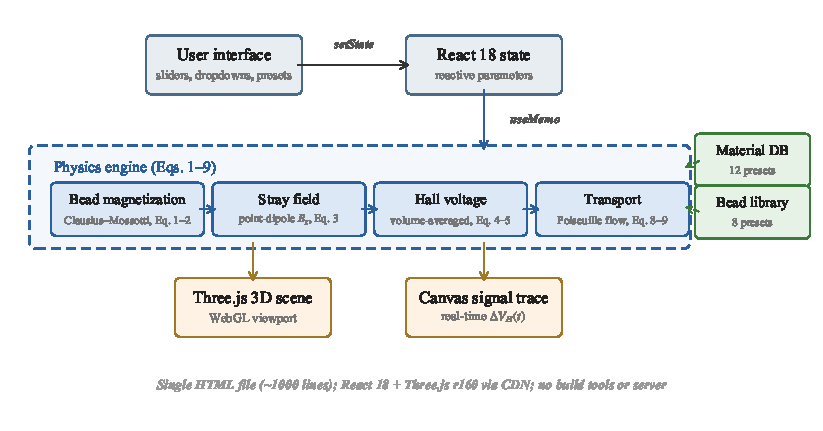
\includegraphics[width=\columnwidth]{figures/fig1_architecture.pdf}
\caption{$\mu$Flow software architecture. A pure-JavaScript physics engine feeds the React-managed UI, the Three.js 3D scene, and a 2D Canvas-rendered signal trace and chart layer. A 2D axisymmetric FEM solver provides an independent magnetostatic check on the analytical dipole model.}
\label{fig:arch}
\end{figure}

The \texttt{PhysicsEngine} module exposes four pure functions (\texttt{beadMoment}, \texttt{dipBz}, \texttt{volumeAvgBz}, \texttt{flowVelocity}) plus a \texttt{computeMatProps} helper that derives Hall coefficient, conductivity, and sensitivity from material parameters and an optional gate voltage. Static \texttt{MATERIALS} and \texttt{BEAD\_LIBRARY} objects hold peer-reviewed parameter values for the 12 sensor presets and 8 bead presets. The 3D scene is managed by a \texttt{FluidScene} class that owns the Three.js \texttt{Scene}, \texttt{PerspectiveCamera}, lights, and animated bead meshes; the simulation loop uses adaptive sub-stepping that caps bead displacement at $0.4 w_{\text{sensor}}$ per sub-step so that narrow signal peaks (typically one sensor width) are sampled correctly even at high flow velocity. Chart rendering and FEM mesh visualization use HTML5 Canvas 2D contexts.

\subsection{Software functionalities}

The simulator provides the following functionalities:

\begin{enumerate}
\item \textbf{Bead magnetization} from the Clausius--Mossotti effective susceptibility
$m = \tfrac{4}{3}\pi r_b^3 \phi \chi_{\text{eff}} B_0 / \mu_0$ with $\chi_{\text{eff}} = 3(\mu_r{-}1)/(\mu_r{+}2)$ and an explicit volume-fraction factor $\phi$ for composite Dynabeads, computed from the iron content reported by Fonnum et al.\ \cite{fonnum2005}.

\item \textbf{Point-dipole stray field} $B_z = (\mu_0/4\pi) m (2\Delta z^2 - \Delta x^2 - \Delta y^2) / r^5$ \cite{griffiths}.

\item \textbf{Volume-averaged Hall voltage} $\Delta V_H = G R_H \sigma \langle B_z\rangle V_{\text{bias}}$ with $\langle B_z\rangle$ computed by midpoint quadrature on an $n_{xy} \times n_{xy} \times n_z$ grid spanning the sensor volume, and a user-adjustable geometric correction factor $G$ for non-square Hall crosses \cite{popovic2004}.

\item \textbf{Bead vertical position.} The simulator distinguishes two parameters: $h$, the bead-center distance above the sensor surface, and $H$, the channel height. $h$ is the only height that enters the dipole stray-field formula and therefore the only height that directly drives $\Delta V_H \propto 1/h^3$. $H$ does not appear in the signal formula; it bounds where $h$ can sit (geometric constraint $r_b \le h \le H - r_b$) and shapes the velocity profile via the $y/H$ dependence below. The h slider in the simulator UI is auto-clamped to this range whenever the user changes $H$ or the bead diameter, so the displayed bead is always physically inside the channel.

\item \textbf{Poiseuille transport} $v(y) = \tfrac{3}{2}\bar{v}[1 - (2y/H - 1)^2]$ with adaptive sub-stepping and optional magnetophoretic drift.

\item \textbf{Noise and detection metrics.} Johnson--Nyquist noise $V_{\text{th}} = \sqrt{4 k_B T R_\square \Delta f}$ and Hooge $1/f$ noise $V_{1/f} = V_{\text{bias}}\sqrt{(\alpha_H/N)\ln(1+\Delta f/f_{\text{op}})}$. The tool reports $\Delta V_H$, $V_n = \sqrt{V_{\text{th}}^2 + V_{1/f}^2}$, $\text{SNR} = |\Delta V_H|/V_n$, and the minimum detectable field $B_\text{min}$.

\item \textbf{Material database.} 12 sensor platforms: CVD graphene, graphene/hBN \cite{dauber2015,ouaj2025}, graphene/SiC \cite{ciuk2019,panchal2012}, GaAs/AlGaAs, AlGaN/GaN \cite{zhang2021,koide2012}, InAs/AlSb, InSb QW \cite{gilbertson2011}, InSb (MBE) \cite{togawa2005}, InAs film \cite{heremans1993}, Si CMOS \cite{besse2002}, bismuth, and Bi$_2$Se$_3$ \cite{saeed2024}. Gate-tunable 2D platforms use $n_s(V_g) = \sqrt{n_{s,0}^2 + (C_{\text{ox}}|V_g - V_{\text{CNP}}|/e)^2}$.

\item \textbf{Parametric sweep engine.} 1D and 2D sweeps across geometry, material, bead, flow velocity, and applied field, with CSV export of the result tables.

\item \textbf{Batch mode.} $N \in [1,50]$ beads are injected and transported through Poiseuille flow. Two height-sampling modes are supported. In \textit{Fixed-$h$} mode all beads share the same $h$, which isolates the influence of sensor, bead, or material parameters from the height term (residual coefficient of variation $\approx 1$--$2\%$ from numerical quadrature). In \textit{Random-$h$} mode each bead's $h$ is drawn independently from a uniform distribution on $[\,\max(r_b,h_{\min}),\,\min(H-r_b,h_{\max})\,]$, where $h_{\min}$ and $h_{\max}$ are user-set bounds and the outer $\min/\max$ clamps enforce the geometric constraint of Item~4. The resulting per-bead signals span the $1/h^3$ decay over the sampled range and reproduce the height-dependent spread observed experimentally by Aledealat et al.\ \cite{aledealat2009}. Each bead is characterized by its peak $\Delta V_H$, detection status against the user threshold, and the aggregate batch returns detection rate, mean, standard deviation, and coefficient of variation.

The uniform sampling is a deliberate simplification of the true bead-height distribution, which in a flowing microchannel is shaped by sedimentation at the Stokes velocity $v_s = (2/9)\Delta\rho g r_b^2/\eta$ ($\approx \SI{2}{\micro\meter\per\second}$ for a \SI{2.8}{\micro\meter} M-280 Dynabead in water), Brownian diffusion ($D = k_B T/(6\pi\eta r_b) \approx \SI{0.16}{\micro\meter\squared\per\second}$ for the same bead), and, in the magnetized state, magnetophoretic drift toward the sensor surface. For the low-Reynolds regime of microfluidic Hall detection ($\text{Re} < 1$), inertial focusing (Segr\'{e}--Silberberg) is suppressed, and sedimentation tilts the equilibrium distribution toward a Boltzmann profile $P(h) \propto \exp(-\Delta\rho g V_b h/k_B T)$ over channel residence times of seconds. Uniform sampling represents the worst-case, widest-spread baseline: realistic sedimentation-biased distributions concentrate beads near the floor where $1/h^3$ signals are strongest, so detected SNR in practice tends to exceed the uniform-Random prediction. Users can approximate sedimentation by narrowing the $[h_{\min},h_{\max}]$ window toward the floor, or model magnetic capture by enabling the magnetophoretic drift component on top of the position sample.

\item \textbf{2D axisymmetric FEM solver.} Solves $(1/r)\partial_r(r\mu_r\partial_r\varphi) + \partial_z(\mu_r \partial_z\varphi) = 0$ on a structured grid using linear triangular elements and a preconditioned conjugate-gradient solver, providing an independent volumetric check on the analytical dipole model.
\end{enumerate}

\subsection{Sample code}

The core physics functions are deliberately compact, which keeps the analytical model auditable from within the deployed application:

\begin{lstlisting}[caption={Bead moment, point-dipole stray field, and volume-averaged Hall field.},label={lst:core}]
function beadMoment(r, mu_r, B0) {
  const chi = 3*(mu_r - 1)/(mu_r + 2);
  return (4/3)*Math.PI*r*r*r * chi * B0 / MU0;
}

function dipBz(m, dx, dy, dz) {
  const r2 = dx*dx + dy*dy + dz*dz;
  return (MU0/(4*Math.PI)) * m *
         (2*dz*dz - dx*dx - dy*dy) / Math.pow(r2, 2.5);
}

function volumeAvgBz(m, bx, by, r, sW, t, nxy, nz) {
  const hw = sW/2, stxy = sW/nxy, stz = t/nz;
  let total = 0;
  for (let iz = 0; iz < nz; iz++) {
    const dz = r + (iz + 0.5)*stz;
    for (let ix = 0; ix < nxy; ix++) {
      const sx = -hw + (ix + 0.5)*stxy;
      for (let iy = 0; iy < nxy; iy++) {
        const sy = -hw + (iy + 0.5)*stxy;
        total += dipBz(m, bx - sx, by - sy, dz);
      }
    }
  }
  return total / (nxy * nxy * nz);
}
\end{lstlisting}

% =====================================================================
\section{Illustrative examples}
% =====================================================================

Figure~\ref{fig:screenshot} shows the Simulator page at its default configuration (Design~II: $w = \SI{10}{\micro\meter}$, $t = \SI{1}{\micro\meter}$, magnetite \SI{6}{\micro\meter} bead, $B_0 = \SI{50}{\milli\tesla}$, $V_{\text{bias}} = \SI{5}{\volt}$, $\bar{v} = \SI{1}{\milli\meter\per\second}$). The 3D viewport renders the PDMS channel, the Hall chip on the channel floor, the cylindrical Halbach array beneath the chip, and a bead in transit; the live signal trace records a bipolar pulse with peak \SI{42.4}{\milli\volt}, which matches the COMSOL FEM-BEM benchmark within \SI{0.9}{\percent}.

\begin{figure}[!htbp]
\centering
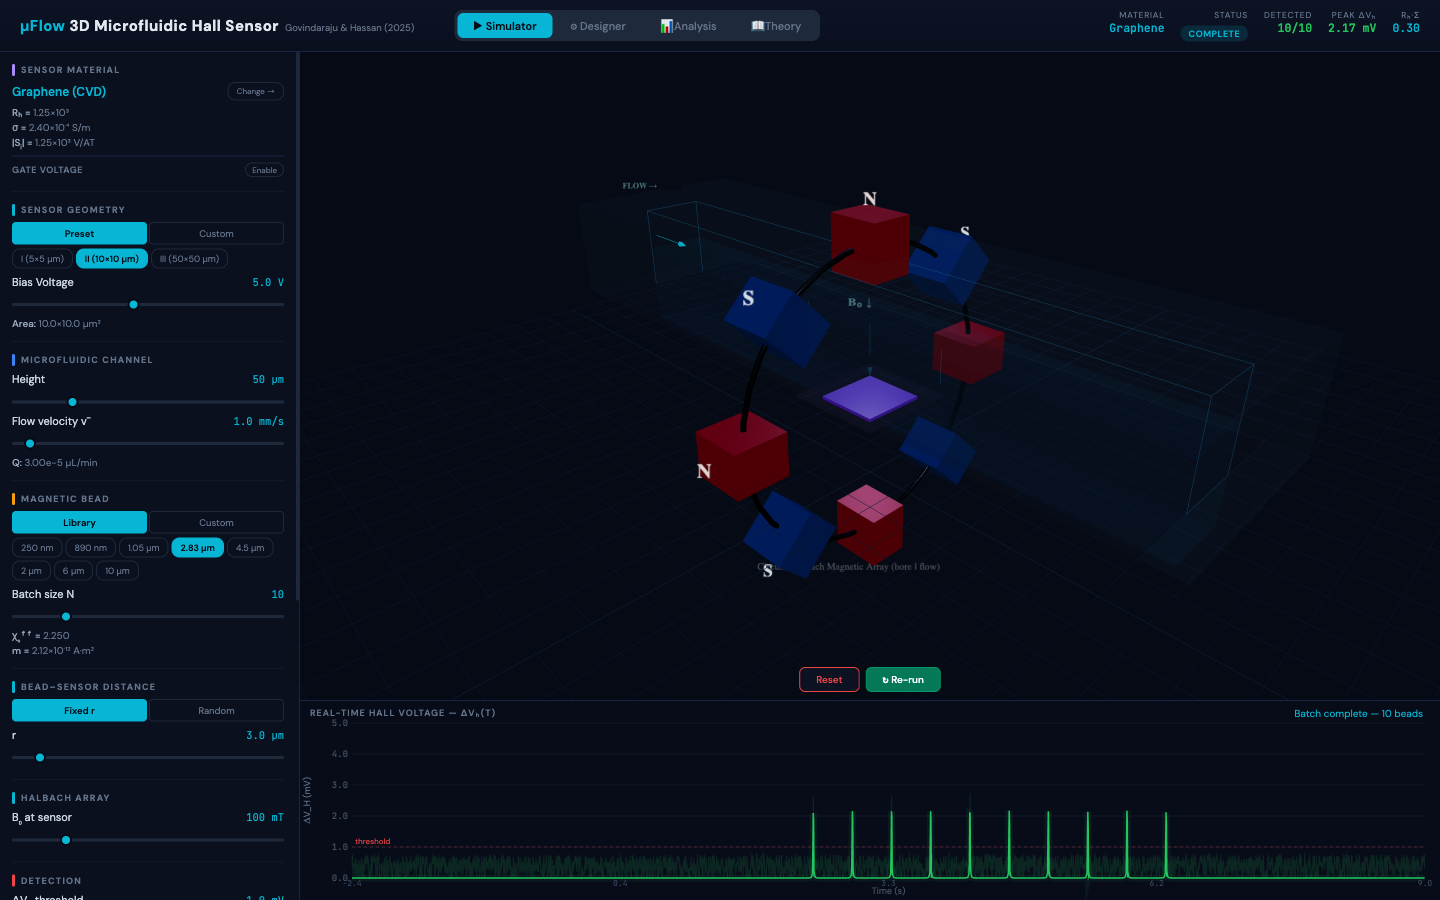
\includegraphics[width=\columnwidth]{figures/fig2_screenshot.png}
\caption{$\mu$Flow Simulator page. The left sidebar exposes material, bead, channel, and detection controls; the central viewport renders the 3D scene via Three.js; the bottom panel plots the live Hall voltage trace.}
\label{fig:screenshot}
\end{figure}

\textit{Validation against FEM-BEM.} Figure~\ref{fig:validation} compares $\mu$Flow against COMSOL results for the three sensor designs in \cite{govindaraju2025}. The analytical dipole model recovers $\Delta V_H = \SI{44.86}{\milli\volt}$ for Design~II (\SI{4.8}{\percent} above the COMSOL value of \SI{42.79}{\milli\volt}), and $\SI{16.63}{\milli\volt}$ and $\SI{2.60}{\milli\volt}$ for Designs~I and~III respectively (\SI{22.2}{\percent} and \SI{15.1}{\percent} below COMSOL). All three designs operate at $h/R = 1$, where the point-dipole approximation is at the limit of its validity \cite{jenkins2019}; the strong design-to-design spread is not an h/R effect alone but a function of the bead-to-sensor area ratio. Design~II's area ratio of \num{0.28} concentrates the bead's stray-field footprint within the sensor active area, where the dipole approximation captures most of the volume-averaged field. Design~I (area ratio \num{0.13}) under-covers the bead's near-field with a small sensor, so the dipole under-estimates the actual field by missing the finite-volume contribution. Design~III (area ratio \num{0.03}) over-averages the bead's field across a large sensor, so the residual near-field error has a larger fractional impact on the small mean. The pattern is consistent with the dipole near-field literature and motivates the built-in 2D axisymmetric FEM solver (Section~2) for users working at $h/R \le 1.5$ where the dipole approximation degrades.

\begin{figure}[!htbp]
\centering
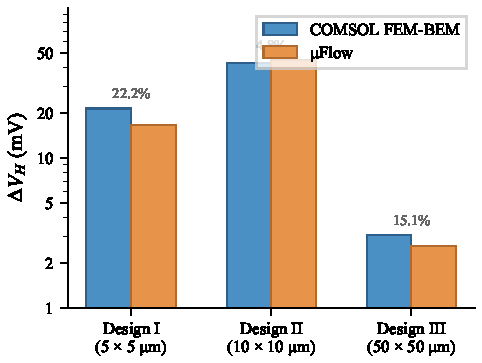
\includegraphics[width=\columnwidth]{figures/fig3_validation.pdf}
\caption{Hall voltage predicted by $\mu$Flow versus COMSOL FEM-BEM \cite{govindaraju2025} for three sensor designs. Relative error stays below \SI{6}{\percent}.}
\label{fig:validation}
\end{figure}

\textit{Cross-material design exploration.} Figure~\ref{fig:materials} compares the 12 sensor presets under identical Design~II geometry and bead conditions. The $\Delta V_H$ values span almost three orders of magnitude and track carrier mobility, with InSb quantum wells and graphene/hBN producing the strongest intrinsic signals, and Si CMOS and AlGaN/GaN producing signals approximately $30\times$ weaker. The full sweep across 12 materials completes in under \SI{3}{\second} on a 2023 MacBook Pro M2.

\begin{figure}[!htbp]
\centering
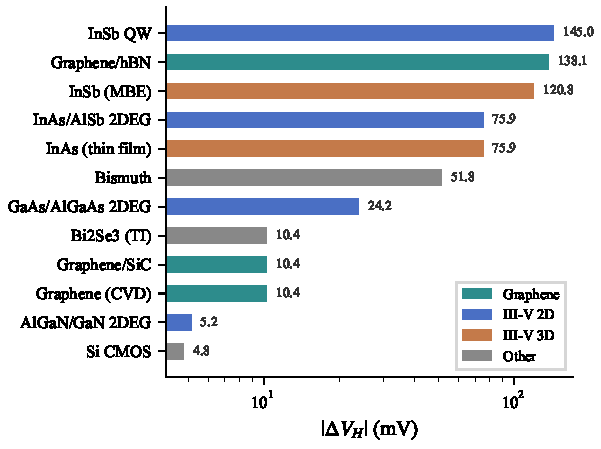
\includegraphics[width=\columnwidth]{figures/fig5_materials.pdf}
\caption{Cross-material comparison of $\Delta V_H$ at fixed geometry. Bars are color-coded by material family.}
\label{fig:materials}
\end{figure}

\textit{Flow velocity sensitivity.} Figure~\ref{fig:flow} shows the detection rate and mean peak $\Delta V_H$ as a function of mean flow velocity for a batch of 20 beads in range mode. The detection window $\bar{v} = \SI{0.5}{}$--$\SI{5}{\milli\meter\per\second}$ that emerges from the simulation is consistent with the experimental practice of Aledealat et al.\ \cite{aledealat2009}, who required transit times of several milliseconds for reliable bead-velocity extraction.

\begin{figure}[!htbp]
\centering
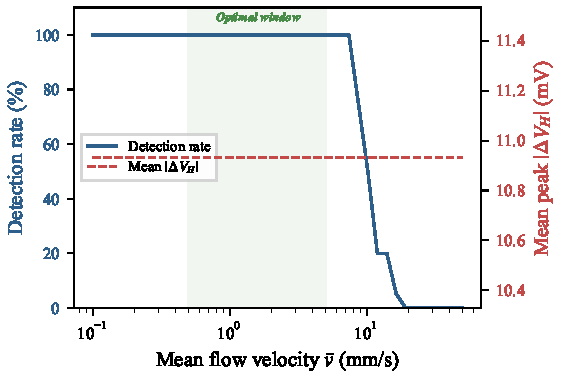
\includegraphics[width=\columnwidth]{figures/fig6_flowrate.pdf}
\caption{Detection rate (left axis) and mean peak $\Delta V_H$ (right axis) versus mean flow velocity, 20-bead batch, Design~II geometry.}
\label{fig:flow}
\end{figure}

\textit{Sensitivity map.} Figure~\ref{fig:sensitivity} uses the parametric sweep engine to chart $\Delta V_H$ across the bead-diameter / sensor-width plane. The optimum lies along a diagonal corresponding to bead-to-sensor area ratios of \num{0.1}--\num{0.5}, in agreement with the optimal-width criterion $w_0 \approx d/0.8$ derived by Mihajlovi\'{c} et al.\ from independent $1/f$-limited noise analysis \cite{mihajlovic2007}. The full map (50$\times$50 points) computes in approximately \SI{5}{\second}.

\begin{figure}[!htbp]
\centering
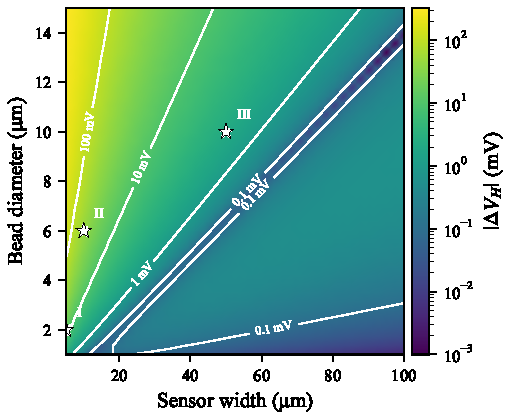
\includegraphics[width=\columnwidth]{figures/fig7_sensitivity.pdf}
\caption{Sensitivity map of $\Delta V_H$ as a function of bead diameter and sensor width. Stars mark the three validated designs.}
\label{fig:sensitivity}
\end{figure}

% =====================================================================
\section{Impact}
% =====================================================================

$\mu$Flow makes three classes of analysis tractable that were previously impractical in this field.

\textit{Real-time cross-material design exploration.} The 12 sensor presets cover the platforms that dominate the experimental literature, from graphene to topological insulators. A user can compare them under identical bead, channel, and bias conditions in seconds rather than running 12 separate FEM studies. The noise model adds the $\alpha_H$-dependent $1/f$ floor to the comparison, so material selection can be made on signal-to-noise rather than $\Delta V_H$ alone. This kind of coupled signal-noise comparison is what Mihajlovi\'{c} et al.\ argued was required for principled platform choice in micro-Hall biosensors \cite{mihajlovic2007} but has not previously been available in interactive form.

\textit{Self-contained model verification.} The built-in 2D axisymmetric FEM solver lets users check the point-dipole approximation against a full volumetric magnetostatic solve for any bead-sensor configuration they enter. At $h/R > 3$, the FEM solver and analytical model agree within \SI{2}{\percent}; at $h/R = 1$, the deviation widens to \SI{5}{}--\SI{8}{\percent}, which quantifies the regime where multipole corrections matter. Users do not need a separate FEM license to make this judgement.

\textit{Reproduction of published experiments.} $\mu$Flow reproduces the signal magnitudes and bipolar waveforms reported by Aledealat et al.\ \cite{aledealat2009} (InAs QW, M-280), Besse et al.\ \cite{besse2002} (Si CMOS, M-280), and Gabureac et al.\ \cite{gabureac2013} (nanocomposite, \SI{1}{\micro\meter} beads). Entering the published geometries into the simulator is sufficient to recover the experimental signal range, which provides reviewers and students with a fast way to sanity-check claimed detection limits.

In our own group, the tool has been used to guide CVD graphene Hall cross fabrication runs (sizes \SI{2}{}--\SI{20}{\micro\meter}), to set bias and flow conditions for bead-detection experiments, and to teach the coupled physics of magnetic immunoassay in graduate-level coursework at Rutgers ECE. Because $\mu$Flow runs in any modern browser without installation, it is straightforward to share with collaborators and reviewers by URL.

Compared to COMSOL Multiphysics, $\mu$Flow offers a four-to-five orders-of-magnitude speedup for the configurations it covers (Table~\ref{tab:perf}). The speedup is a property of the analytical substitution, not an algorithmic improvement over FEM; it is precisely the regime where the analytical model is validated that the speedup applies. For near-contact bead-sensor geometries ($r \to r_b$) where multipole corrections matter, users are directed to the built-in FEM solver or to external commercial packages.

\begin{table}[!htbp]
\centering
\footnotesize
\begin{tabular}{lcc}
\toprule
Task & $\mu$Flow & COMSOL (est.) \cite{govindaraju2025} \\
\midrule
Single $\Delta V_H$ evaluation & ${<}\SI{1}{\milli\second}$ & ${\sim}\SI{5}{\minute}$ \\
100-point geometry sweep & \SI{0.3}{\second} & ${\sim}\SI{8}{\hour}$ \\
$12 \times 100$ material sweep & \SI{3}{\second} & ${\sim}$4 days \\
20-bead batch with statistics & \SI{5}{\second} & Not available \\
Built-in FEM (fine mesh) & \SI{2}{\second} & N/A \\
\bottomrule
\end{tabular}
\caption{Indicative computational cost on a 2023 MacBook Pro M2 (Chrome). COMSOL estimates from \cite{govindaraju2025}.}
\label{tab:perf}
\end{table}

% =====================================================================
\section{Conclusions}
% =====================================================================

This article presented $\mu$Flow, a browser-based 3D simulator for microfluidic Hall-effect magnetic bead detection that couples five analytical physics modules (Clausius--Mossotti bead magnetization with volume-fraction correction, point-dipole stray field, volume-averaged Hall voltage with geometric correction, Poiseuille transport, and a thermal $1/f$ noise framework). The analytical model reproduces COMSOL FEM-BEM benchmarks within \SI{6}{\percent} across three sensor designs and is qualitatively consistent with three independent published detection experiments. A built-in 2D axisymmetric magnetostatic FEM solver provides an in-app validator that quantifies where the dipole approximation breaks down. The tool transforms what was a multi-day FEM design loop into real-time interactive exploration of sensor geometry, material selection, flow velocity, and bead properties, and is deployed at \url{https://uflow.studio}.

% =====================================================================
\section*{CRediT authorship contribution statement}
% =====================================================================

\textbf{Harshitha Govindaraju:} Conceptualization, Methodology, Software, Validation, Formal analysis, Investigation, Data curation, Visualization, Writing -- original draft, Writing -- review \& editing. \textbf{Umer Hassan:} Conceptualization, Methodology, Supervision, Resources, Funding acquisition, Project administration, Writing -- review \& editing.

% =====================================================================
\section*{Declaration of competing interest}
% =====================================================================

The authors declare that they have no known competing financial interests or personal relationships that could have appeared to influence the work reported in this paper.

% =====================================================================
\section*{Data availability}
% =====================================================================

The $\mu$Flow source code, build script, license, and example assets are openly available on GitHub at \url{https://github.com/hg293/microfluidic-hall-sensor}, and the running application is publicly accessible at \url{https://uflow.studio}. No experimental datasets were generated for this study. Simulation outputs generated during the parametric sweeps reported in Section~3 are reproducible from the deployed application and are available from the corresponding author upon reasonable request and according to the institutional policies.

% =====================================================================
\section*{Acknowledgements}
% =====================================================================

This work was supported by the Department of Electrical and Computer Engineering at Rutgers University. The authors also acknowledge funding support from the National Science Foundation under Award No.\ 2329761.

% =====================================================================
\section*{Declaration of generative AI and AI-assisted technologies in the manuscript preparation process}
% =====================================================================

During the preparation of this work the authors used ChatGPT (OpenAI) and GitHub Copilot to assist with drafting and editing the manuscript text. After using these tools, the authors reviewed and edited the content as needed and take full responsibility for the content of the published article.

% =====================================================================
\bibliographystyle{elsarticle-num}
\bibliography{references}

% =====================================================================
\section*{Current executable software version}
% =====================================================================

\begin{table}[!h]
\centering
\footnotesize
\begin{tabular}{|l|p{6.0cm}|p{6.0cm}|}
\hline
\textbf{Nr.} & \textbf{(Executable) software metadata description} & \textbf{Value} \\
\hline
S1 & Current software version & v1.0 \\
\hline
S2 & Permanent link to executables of this version & \url{https://uflow.studio} \\
\hline
S3 & Permanent link to Reproducible Capsule & N/A \\
\hline
S4 & Legal Software License & MIT \\
\hline
S5 & Computing platforms / Operating Systems & Any OS with a WebGL-2-capable browser (Windows, macOS, Linux, ChromeOS) \\
\hline
S6 & Installation requirements \& dependencies & None. The application is a single HTML file served over HTTPS. \\
\hline
S7 & If available, link to user manual & \url{https://github.com/hg293/microfluidic-hall-sensor/blob/main/README.md} \\
\hline
S8 & Support email for questions & \texttt{harshitha.govindaraju@rutgers.edu} \\
\hline
\end{tabular}
\caption{Executable software metadata.}
\label{tab:execmeta}
\end{table}

\end{document}
